\documentclass[11pt, a4paper, oneside,titlepage]{article}
\usepackage{times}
\usepackage{graphicx}
\usepackage{epsfig}
\usepackage{amssymb}
\usepackage{amsmath}
\usepackage{amsthm}
\usepackage{epstopdf}
\usepackage{url}
\usepackage{amsmath}
\usepackage{mathtools}
\usepackage{fixltx2e}
\usepackage[top=1.5in, bottom=1in, left=1in, right=1in]{geometry}
\usepackage{parskip}
\usepackage{framed}
\usepackage{enumitem}
\usepackage{amssymb}

% Proof Style

\renewcommand\abstractname{\textit{Abstract}}
\newcommand{\HRule}{\rule{\linewidth}{0.4mm}}

\renewcommand{\familydefault}{\rmdefault}
\renewcommand{\rmdefault}{cmr}
\normalfont





\begin{document}
\begin{titlepage}
\begin{center}
	\textsc{\LARGE Imperial College London}\\[1.5cm]

	\textsc{\Large Department of Computing}\\[0.5cm]

	\HRule \\[0.4cm]
	{\LARGE \bfseries On-the-fly Modelling and Prediction of Epidemic Phenomena \\[0.4cm] }
	\HRule \\[1.5cm]

\begin{minipage}{0.4\textwidth}
\begin{flushleft} \large
\emph{Author:}\\
James \textsc{Hay}
\end{flushleft}
\end{minipage}
\begin{minipage}{0.4\textwidth}
\begin{flushright} \large
\emph{Supervisor:} \\
Dr.~William \textsc{Knottenbelt}
\end{flushright}
\end{minipage}
\vfill

\includegraphics[width=5cm]{ImperialCrest.jpg}
\vfill
Submitted in partial fulfilment of the requirements for the MSc Degree in Computing Science of Imperial College London
\vfill
% Bottom of the page
{\large September 2014}
\end{center}
\end{titlepage}

\section*{Abstract}


\newpage
\section*{Acknowledgements}
I would like to thank all my mates who without my mates I would not be
able to do my project, like at all.

\newpage
\section{Introduction}
\subsection{Overview}
This project provides a framework with which the dynamics of
an epidemic event composed of multiple, overlapping sub-epidemics may be modelled and
forecasted in real time. We aim to provide an optimised model fit to a
given set of epidemic data where all model parameters are assumed to
be unknown. The challenge of considering various candidate model
types is also considered. Unlike previous approaches, the presented framework is
implemented in object oriented style using a general purpose
programming language, allowing improved customisability and
speed. Furthermore, we attempt to implement a maximum likelihood based
fitting procedure, which has previously only been considered for
single epidemic models.


\subsection{Motivation}
Epidemic spreading processes can be observed in a wide range of
fields. Any type of interaction between individuals will allow the
propogation of ideas or parasites through a population, with some spreading
processes arising unexpectedly in excess of baackground levels. In the case of
infectious diseases, such outbreaks are termed epidemics. Indeed, many significant
historical events have been heavily influenced by epidemics, and the
WHO estimates that infectious diseases account for more than 13
million deaths per year.\cite{who} It is therefore no wonder that
epidemiology, the study of the mechanisms and population dynamics of
infectious diseases, has become a central field of research. With the
advancement of computing technology and methodology, new opportunities
to develop complex mathematical and computational models of real-time
epidemics have emerged.

Although the study of infectious disease spread continues to be an
area of particular research focus, globalisation and advances in
communication technologies have led to a new and rapidly developing
type of internet based epidemic. With the entire world connected
online, new ideas, trends and information can disseminate through the
world wide web almost instantaneously, and as these spreading
processes become increasingly central to modern day life, interest
from academic, commercial and social fields continues to increase. One
highly relevant theory is that of `memes' as proposed by Richard
Dawkins, who suggests that ideas, behaviours and styles spread like
"mind viruses" between individuals within a culture.\cite{dawkins} The
adaptation of this term to describe the spread of fads on the internet
demonstrates the relevance of studying the dynamics of epidemic
processes over the internet. \cite{meme}

Research into the dynamics of internet-based phenomena are largely at
an early stage, and have mostly focused on Online Social Networks
(OSNs) such as Facebook and Twitter, and content sharing websites such
as YouTube.\cite{hartmann, bieber} The analogy between infectious
diseases and the spread of content online is easy to consider: the
social networks formed on OSNs simulate physical interactions in real
life as users interact and share content on their profiles, whilst
viewing and subsequently sharing a YouTube video may be compared to
contracting and spreading an infectious disease. There is a growing
body of research that aims to use ideas from epidemiology to better
understand the spread of internet-based phenomena. \cite{marily2013,
  meme, wang} Taking inspiration from epidemiology, the study of
internet-based epidemic phenomena has investigated the applicability
of both locally and globally driven models. For example, some studies
have investigated the use of diffusion models to describe the
disemmination of influence, whilst others have investigated the use of
global mathematical models.\cite{marily2013, meme, wang, hu}

Whilst these studies have shown generally promising results, a recent
study highlighted the limitations of the single epidemic based
approach.\cite{marily2013} The co-occurence and interaction between
diseases and with environmental factors is increasingly realised as
important, and the authors suggest that the corresponding field of
\emph{synepidemiology} can be applied to internet-based
epidemics.\cite{singer, bastos} The authors go on to coin the term
\emph{synthedemics} to describe the co-occurence of a set of
infections that may or may not be dependent on each
other.\cite{marily2014} Taking inspiration from Fourier analysis, the
study goes on to investigate how an incoming epidemic signal can be
broken down and described in terms of multiple epidemic components
(Figure 1). Furthermore, the authors build on a previous study to
allow models to be fit in real time without making assumptions
regarding the initial model parameters.




 \begin{figure}[ht!]
\centering
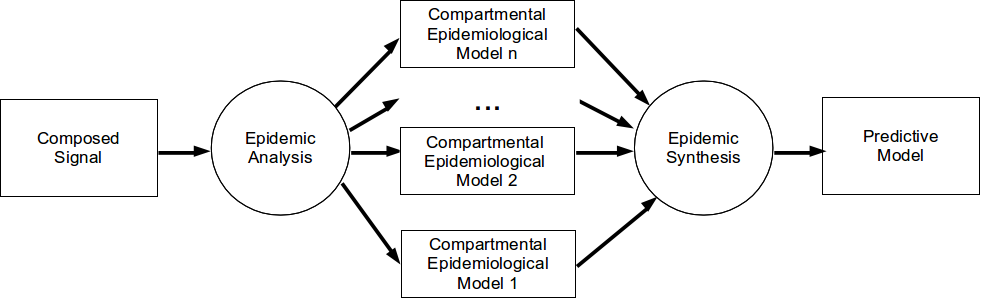
\includegraphics[width=140mm]{marily2014.png}
\caption{Model construction framework as proposed by Nika et al. 2014.\cite{marily2014}}
\label{sir}
\end{figure}



\subsection{Objectives}
The aim of this project is to implement a real time model fitting
framework with which epidemic phenomena might be characterised and
forecasted. When provided with epidemic data up to an arbritary time point,
we attempt to fit an appropriate number of sub-epidemics of various
types to best describe the current data, and to allow future time
points to be predicted. The course of the project can be split up into
the following sub goals:

\subsubsection{Single Epidemics}
The first objective of this project is to implement a single epidemic
fitting framework, treating the growth and recovery rates of the
epidemic as unknown parameters. This framework is then extended to
additionally consider the initial number of susceptible individuals
and the actual epidemic start time as unknown parameters. The model
fitting procedure is undertaken using optimisation with both least
squares and maximum likelihood estimations. The framework allows for
`on the fly' fitting, such that a model may be fit to the data as the
epidemic unfolds and more data points are obtained.

The initial implementation of this framework is initially undetaken using the R
statistics programming environment due to the availability of useful
packages and functions. For example, the \emph{deSolve} for solving
first-order ordinary diffierential equations (ODEs), the \emph{optim}
function for optimising a set of model parameters, and the
\emph{bbmle} package for maximum likeliihood based fitting.

An extension of this objective that arose during the course of the
project is the implementation of the fitting framework in C++ `from
scratch'.

\subsubsection{Multiple Epidemics}
Not all epidemic phenomena are constrained to a single population, and
the single epidemic fitting methodology is therefore inadequate in
characterising all epidemics. For example, the measure of
\emph{YouTube} video views over time might be composed of multiple
spikes of interest as the video is shared in new online social
groups. This limitation also affects to infectious disease dynamics,
wherein the total number of infected individuals in a country might be
affected by the penetration of the disease into different cities. The
second objective of this project is therefore to implement a model
fitting framework that can simultaneously fit and combine multiple
sub epidemics into a single model. 

As in the single epidemic fitting framework, the multiple epidemic
fitting framework makes no assumptions regarding model parameters such
as growth rate, recovery rate, start time and number of
susceptibles. As above, an initial implementation will be attempted
using R. However, as the computational difficulty of fitting
multiple sets of parameters simultaneously increases as the number of
sub epidemics increases. We therefore provide a final `from scratch' implementation in C++.

A significant extension of this fitting methodology is to allow
different epidemic models to be considered. That is, which one of a
number of model equations can be used to best describe the data? An
object-oriented C++ implementation is therefore provided to consider
the addition and removal of various candidate models to describe a set
of data.

\subsubsection{Maximum Likelihood Estimation}
A novel objective of this project is to use maximum likelihood rather
than least squares to find an optimised model fit. A significant
challenge of this is to implement an efficient likelihood function in
C++ with which a set of parameters might be optimised in reasonable
time. An advanced extension of this objective is to generate confidence
intervals characterise uncertainty in the optimised parameters. 

\subsubsection{Evaluation}
All of the above objectives must be validated, and we use a
number of data sources to assess the model fitting
framework. Synthetic data provides the core of the evaluation, as it
allows for the retrieval of known parameters from artificially
generated data. Finally, we consider the framework's ability to
provide model fits to historic infectious disease data and online
epidemic phenomena.


\subsection{Contributions}


\subsection{Report Structure}

\newpage
\section{Background}
\subsection{Modelling Infectious Disease Dynamics}
Throughout history, infectious diseases can consistently be cited as one of the leading causes of death across the world. Whilst many such diseases may be endemic in a population,  a large proportion  of diseases may outbreak as epidemics. That is, a disease may arise in a community, region or even worldwide in excess of normal levels following a particular outbreak. In an age of increasing urbanisation, global connectivity and a larger immuno-compromised population, monitoring and controlling the spread of epidemics is absolutely paramount.\cite{computational} Recent events such as the 2009 flu pandemic highlight the incredible need for a solid understanding of the underlying mechanisms of such diseases. This section will discuss the history and current standards in epidemiology.

A general understanding of infectious disease behaviour can be seen as early as the 8th century A.D., when the Indians and Chinese used a rudamentary form of vaccination known as variolation to control smallpox.\cite{variolation} Even earlier than this, Hippocrates (c. 460-c. 370 BC) was amongst the first to propose that disease spread could be explained rationally through human behaviour and environmental factors.\cite{hippo} Unfortunately, the understanding of infectious disease dynamics appeared to regress until the 17th century when the collection of the first public health statistics allowed for a more scientific approach. 

One of the first predictive mathematical models was by Bernoulli in 1760, who used mathematical techniques to establish that variolation for smallbox could help increase the life expectancy in the French population.\cite{brauer} Similarly, another systematic study of disease dynamics took place in 1854 by John Snow, who identified a single water pump in London as the likely source of a Cholera epidemic.\cite{snow} However, it was the early 1900s in which the most fundamental advances in mathematical epidemiology were made. Firstly by Ross in 1911, who used a spatial model to describe the spread of malaria due to mosquitoes.\cite{snow} This study was the first to demonstrate that infectious diseases could be controlled by reducing the population of infected individuals below a certain threshold. The next and arguably most central breakthrough was then made by Kermack and McKendrick in 1927, who proposed the use of ordinary differential equations (ODEs).\cite{kermack} ODEs represented the first deterministic, general epidemic model to describe mass action. The general idea behind ODE models in the context of epidemiology is that individuals in a given population are members of various compartments depending on their relationship to the infection (eg. infected, recovered), and individuals switch between compartments as described by these ODEs.

The most basic form of the model prosed by Kermack and McKendrick's ODEs is the Susceptible-Infected-Recovered (SIR) model. Given a population of size N, individuals are divided into three states or compartments: 

\begin{enumerate}
	\item Individuals that are susceptible to the infection, denoted by $S(t)$
	\item Individuals that are infected with the disease and are therefore capable of infecting others, denoted by $I(t)$
	\item Individuals that have been removed from the population or recovered, denoted by $R(t)$. 
\end{enumerate}

Individuals move between compartments in the following order:
\begin{equation*}
S \Longrightarrow I \Longrightarrow R
\end{equation*}
Simply, individuals start off as being free of the disease, but susceptible to infection. Individuals are then infected with the disease and begin to display symptoms, thereby becoming infectious themselves. After a certain period of time, individuals are no longer infectious as they recover and become immune to the disease. In this model, the population size is assumed to be fixed such that:

\begin{figure}[ht!]
\centering
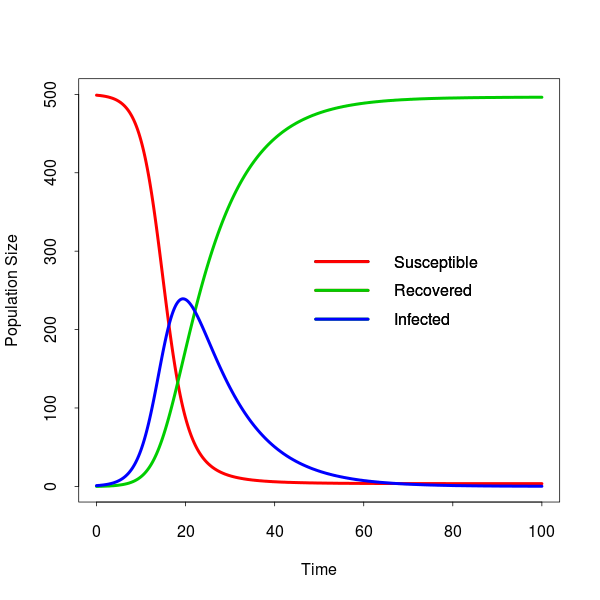
\includegraphics[width=120mm]{Rplot.png}
\caption{Generic example of the classic SIR model demonstrating the change in population size for each compartment as the epidemic unfolds}
\label{sir}
\end{figure}

\begin{equation*}
N = S(t) + I(t) + R(t)
\end{equation*}

The way in which individuals individuals move between these compartments are described by the following set of ODEs:
\begin{equation*}
	\begin{split}
	&\frac{dS}{dt} = -\beta IS, \\
	&\frac{dI}{dt} = \beta IS - \gamma I, \\
	&\frac{dR}{dt} = \gamma I
	\end{split}
\end{equation*}

The dynamics of these ODEs are influenced by two key parameters: the contact rate, $\beta$, and the recovery rate, $\gamma$. $\beta$ describes the probability of an infected person coming into contact with any susceptible person per unit time, whereas $\gamma$ describes the rate at which an individual recovers from the disease. When $\beta$ is large, the contact rate between individuals is high, and the disease spreads rapidly. Similarly, when $\gamma$ is large, then individuals recover rapidly and move to the recovered compartment quickly. Note that these parameters make global assumptions about the population, in that all individuals have an equal chance of interacting, and all individuals recover at the same rate. Infected individuals therefore come into contact with $\beta$$N$ individuals per unit time. Only susceptible individuals may become infected, and the number of new infections per unit time is therefore $\beta$$N(S/N)$, resulting in a new infection rate of $\beta$$N(S/N)I = $$\beta$$SI$. Finally, as individuals recover with rate $\gamma$, they are removed from the infected compartment and enter the recovered department with rate $\gamma I$.

Considering these parameters allow for useful insights into the dynamics of a given disease: a disease with a high $\beta$ and lower $\gamma$ will obviously spread more than one with a lower contact rate and higher recovery rate. With this in mind, we can make the intuitive leap to conclude that an infection will either: spread as an epidemic when each individual is causing more than one secondary infection; remain endemic in a population when each individual causes exactly one further infection before recovering; will die out when each individual causes less than one secondary infection before recovering. This idea is formalised by the concept of a \emph{basic reproductive number}, $R_0$ (not to be confused with $R(0)$, which denotes the initial size of the recovered population!). $R_0$ denotes the number of secondary infections caused by a single infected individual when introduced into an initial susceptible population, $S(0)$. As this infected individual will come into contact with $\beta N$ individuals per unit time over a period of $1/$$\gamma$ (the mean infectious period), the reproductive number will be given as the number of secondary infections per unit time multiplied by the amount of time that an individual can infect others:\cite{anderson, diekmann}

\begin{equation*}
R_0 = (\beta N)/\gamma
\end{equation*}

$R_0$ describes the number of secondary infections resulting from one individual in a completely susceptible population; however, this rate will obviously decrease as the proportion of susceptible individuals in the population decreases. Rather than considering the initial reproductive number, it is often more useful to consider the effective reproduction number, $R_n$ . In simplest terms, $R_n = R_0 \times s$, where $s$ is the proportion of the population that is susceptible ($S(t)/N$).

As an aside, it should be noted that calculating $R_0$ is a crucial stage in understanding how a disease will spread. A high $R_0$ (eg. malaria) means that the disease will spread rapidly, with each individual causing a high number of secondary infections, whereas a low $R0$ (eg. monkeypox) means that a disease will spread slowly.\cite{vynnycky} As discussed above, an $R_0$ greater than 1 is necessary for an epidemic to take hold. Even at an early stage of an epidemic, $R_0$ can be estimated based on the growth rate of an epidemic, as was the case during the 2003 SARS virus.\cite{sars} Therefore, decreasing the proportion of sucseptible individuals below a certain level (ie. through vaccination) will result in an effective reproduction number of less than 1, preventing the epidemic from taking hold. This critical threshold is defined as the \emph{herd immunity threshold}, and provides a crude but often effective target for immunization programmes:\cite{cockman}

\begin{equation*}
HIT = 1 - \frac{1}{R_0} = \frac{R_0 -1}{R_0}
\end{equation*}

The model shown above describes three compartments, however there are a number of extensions to this model where different compartments and interactions might be appropriate. For example, an "exposed" compartment might be added which encompasses individuals that have been exposed to the disease, but are not yet infectious. Such a model is known as the SEIR model. As well as additional compartments, the transitions between these compartments might be varied. For example, in cases where immunity is only transient, individuals might be able to re-enter the susceptible compartment following recovery (the SIRS model). Choosing the model structure is dependent on the nature of the disease and population under consideration. For example, using an SIS (infected individuals return to the susceptible state) to model HIV, or an MSIR model (initial maternal-derived immunity) in the case of measles.\cite{vynnycky} 

It should be noted that there are further considerations to take when modelling real epidemics. For example, the inclusion of birth and death rate, seasonal dynamics, stochasticity and age-dependent interactions.\cite{vynnycky} However, the basic principles discussed above are sufficient to begin considering how we might model the spread of other epidemic processes. 

With the solid theoretical basis described above, advanced mathematical and computational models are becoming increasingly central to making public health decisions. One recent application of mathematical models in epidemiology was to describe and predict the dynamics of an epidemic in real time.\cite{kerkhove} A study by Tizzoni et al. used a Monte Carlo Maximum Likelihood (MCML)-based approach on historical data from the 2009 flu pandemic to develop a global stochastic simulation model, referred to as GLEAM, to obtain basic model parameters.\cite{gleam, gleam2} (Note that this project will aim to similar methodologies to fit epidemic models in real time, and a brief overview of maximum-likelihood estimation and least squares estimation is provided in Box 1). Tizzoni et al. used GLEAM to estimate the seasonal transmission ability of the 2009 H1N1 pandemic, generating forecasts for the activity peaks in the northern hemisphere. The robustness of this stochastic forecast was also explored as a function of data completeness by fitting the model using only partial data.\cite{tizzoni} 

Tizzoni et al. showed that the GLEAM model was in good agreement with the actual 2009 epidemic data, even when only partial data was used (for example, pre-exposure immunity and adherence to vaccination campaigns. However, a key feature of the model is that it accounts for the way in which  populations interact and connect, and it was shown that model accuracy was reduced considerably when using only a partial dataset for population mobility. The GLEAM model uses three layers: a population layer (a grid representing the population of the world); a mobility layer (using real flight data to represent travel between cells in the grid); and an epidemic model (consisting of susceptible, latent, symptomatic infectious able to travel, symptomatic infectious unable to trabel, asymptomatic infectious and permanently covered compartments). Indeed, consideration of multiple networks layers in epidemic modelling is a growing area of consideration for real infectious diseases, as it alows for the consideration of more realistic population dynamics.\cite{gefm} \\\\

\subsection{Development Environment}
\subsubsection{Programming Languages}
There were a number of candidate programming languages, each with
their own strengths and weaknesses. In the end, R and C++ were chosen
for intitial and final implementations. Previous
approaches to epidemic and synthedemic model fitting frameworks use R
due to its readily available ODE solvers, optimisation functions and
graph plotting functionality.\cite{marily2013,marily2014} R therefore
provided an ideal means to implement the single and multiple epidemic
fitting frameworks initially. Once this initial model fitting
framework was implemented, we went on to provide a C++ implementation
with the aim of providing a faster, more transparent `from scratch'
fitting methodology.

At the start of the project, it was desirable to begin exploring and
understanding the theory behind epidemic modelling and otpimised model
fitting. As such, the first development consideration was to decide on
a language that was well adapted for easy implementations with a large
number of available packages and functions. R and Matlab were
candidates for this initial approach. Whilst Matlab has an arguably
better programming environment with better documentation, R has
already been shown to be effective in epidemic model fitting. The R
community provides a number of statistical analysis tools and is suited to dealing with non-typed data
sets, making it an ideal choice. These packages can easily be obtained
via the Comprehensive R Archive Network (CRAN).

The nature of parameter optimisation means that fitting a large number
of parameters simultaneously can be extremely slow, and an approach to
providing a faster implementation was to reimplement the model fitting
procedure in C++. C++ has been shown to be considerably faster than
both R and Matlab when solving stochastic neoclassical growth models,
suggesting that an efficient C++ implementation might provide a much
faster fitting framework than an R counterpart.\cite{languagespeed}
However, the trade off with run time speed is the fact that coding the
same algorithms and functions in C++ is very time consuming. Whilst
there are R packages readily available that allow parameter fit optimisation,
maximum likelihood estimations and graph plotting in only a few lines
of code, the equivalent functionality in C++ had to be implemented
from scratch. A significant challenge of this project was therefore to
find, adapt or create source code for the essential functions of the
model fitting framework. For graph plotting, a Gnuplot iostream was called from C++
code. 

Python and Java were also considered as potential languages for a
faster implementation. However, the relatively lower speed of Python and
unfamiliarity with Java meant that C++ remained the ideal choice.

It should be noted that whilst C++ provides an ideal way of speeding
up computational bottlenecks in the model fitting procedure (namely
the optimisation step), it it may still be desirable to call R
functions from within the C++ program. For example, the generation of
a likelihood profile. This can be achieved using the
Rcpp library if needed. Furthermore, the quick generation of synthetic
data with which to evaluate and develop the fitting framework is
clearly not a limiting factor. R therefore remained the ideal language
for syynthetic data generation using \emph{GillespieSSA} package,
exporting the data as a .csv file to be imported in the C++ implementation. 

 
 
\newpage
\section{Single Epidemic Fitting}
In this section we explore the theory and implementation behind a
model fitting framework for single SIR models with unknown
parameters. To provide a simulation of real time model fitting, we
iteratively fit a new optimised model at each data point. Firstly, a
least-squares fitting procedure is implemented in R for a single SIR
epidemic where beta, gamma and S0 are assumed to be entirely
unknown. We then extend the implementation to include the start time
of the epidemic, t0 as a fourth unknown parameter. This also raises
the issue of epidemic outbreak detection and model selection, which we
will revisit in section SECTIONNNN!. We go on to use a maximum
likelihood based approach which allows for the generation of
confidence intervals. Finally, we reimplement the above approaches in
C++ to provide a much faster implementation.



\subsection{Parameter Optimisation}
As discussed in SECTION BACKGROUND, the ultimate aim of the
optimisation procedure is to find the set of parameters for a set of
ODEs that, when solved, best fit the given data. 

\subsubsection{The Nelder-Mead Algorithm}

\subsection{}



\newpage
\section{Multiple Epidemic Fitting}


\newpage
\section{Evaluation}


\newpage
\section{Conclusions and Future Work}

\begin{thebibliography}{1}
	\bibitem{who}
		World Health Organisation,
		\emph{Major causes of death}.
		2014,
		Available at \url{http://www.who.int/mediacentre/factsheets/fs310/en/index2.html}
	\bibitem{dawkins}
		Dawkins, R (1976) The Selfish Gene. Oxford University Press, Oxford, UK.
	\bibitem{hartmann}
		W. Hartmann, P. Manchanda, H. Nair, M. Bothner, P. Dodds, D. Godes, K. Hosanagar, and C. Tucker. Modeling Social Interactions: Identification, Empirical Methods and Policy Implications. \emph{Marketing Letters}, 19(3):287-304, December 2008.
	\bibitem{bieber}
		V. Tweedle and R. J. Smith. A mathematical model of Bieber Fever: The most infectious disease of our time. Understanding the dynamics. March 2012
	\bibitem{marily2013}
		M. Nika, G. Ivanova, WJ. Knottenbelt (2013) On celebrity, epidemiology and the internet. In: Proc. 7Th International Conference on Performance Evaluation Methodologies and Tools (VALUE-TOOLS). Turin, Italy
	\bibitem{meme}
		C. Bauckhage, K. Kersting, and F. Hadiji. Mathematical Models of Fads Explain the Temporal Dynamics of Internet Memes. In Proc. ICWSM. AAAI, 2013.
	\bibitem{wang}
	H. Li, H. Wang, J. Liu, and K. Xu. Video sharing in online social networks: measurement and analysis. In \emph{Proceedings of the 22nd international workshop on Network and Operating System Support for Digital Audio and Video}, NOSSDAV '12, pages 83-88, New York, NY, USA, 2012. ACM
	\bibitem{hu}
		H.-W. Hu and S.-Y. Lee. Study on inuence diffusion in social network. \emph{International Journal of Computer Science and Electronics Engineering} (IJCSEE), 1, 2013.
	\bibitem{singer}
		M. Singer, \emph{Introduction to Syndemics}. Wiley.
	\bibitem{bastos}
		F. Bastos et al. Co-infection with malaria and HIV in injecting drug users in Brazil: A new challenge to public health? \emph{Addition} 94:1165-174, 1999
	\bibitem{marily2014}
	M. Nika, T. Wilding, WJ. Knottenbelt. Going Multi-Viral: Synthedemic Modelling and Prediction of Internet-based Phenomena. \emph{In press}
	\bibitem{computational}
	M. Marathe and A. K. S. Vullikanti. Computational
        epidemiology. \emph{Commun. ACM}, 56(7):88-96, July 2013.
        \bibitem{languagespeed} S. Boraan Aruoba,
          J. Fernandez-Villaverde. A Comparison of Programming
          Languages in Economics. \emph{NBER Working Paper} No. 20263,
          June 2014.
	\bibitem{variolation}
	G. Williams (2010). \emph{Angel of Death}. Basingstoke: Palgrave Macmillan.
	\bibitem{hippo}
	F. Adams, E. Kelly (2006) \emph{The Genuine Works of Hippocrates}. Kessinger Publishing. URL http://books.google.co.uk/books?id=X7uR4S5YvhQC
	\bibitem{brauer}
	 Brauer, F., van den Driessche, P. and Wu, J. editors.  Mathematical Epidemiology. \emph{Lecture Notes in Mathematics}. Springer Verlag, 1945 
	\bibitem{snow}
	J. Snow (1855) \emph{On the Mode of Communication of Cholera}. John Churchill. URL http://books.google.co.uk/books?id=-NO\_AAAAcAAJ.
	\bibitem{kermack}
	WO. Kermack, AG. McKendrick (1991) Contributions to the mathematical theory of epidemics-I. 1927. \emph{Bull Math Biol} 53: 33-55.
	\bibitem{vynnycky}
	E. Vynnycky, R. White (2010) An Introduction to Infectious Disease Modelling.
	\bibitem{anderson}
	RM. Anderson, RM. May (1991) Infectious Diseases of Humans: Dynamics and Control. \emph{Oxford University Press}
	\bibitem{diekmann}
	O. Diekmann, JAP. Heesterbeek, JAJ Metz. On the definition and the computation of the basic reproduction ratio $R0$ in models for infectious diseases in heterogenous populations. \emph{Journal of Mathematical Biology} 1990:28;365-382
	\bibitem{goffman}
	D. J. Daley and D. G. Kendall. Epidemics and rumours. \emph{Nature}, 204(4963):1118-1118, 12 1964
	\bibitem{cannarella}
	Cannarella, J and Spechler, JA (2014) Epidemiological Modeling of Online Social Network Dynamics. arXiv:1401.4208 [cs.SI]
	\bibitem{facebook}
Develing, M; Adamic, L; Taylor, S. Debunking Princeton. URL: https://www.facebook.com/notes/mike-develin/debunking-princeton/10151947421191849
	\bibitem{facegroup}
	Facegroup. How stuff spreads: How videos go viral part I. URL: http://www.facegroup.com/how-videos-go-viral.html	
	\bibitem{bisset}
	K. Bisset et al. Interaction-based HPC modeling of social, biological, and economic contagions over large networks. In \emph{Proc. of Winter Simulation Conference} (2011), 2933-2947.
	\bibitem{turner}
	J. Turner, M. Begon, RG. Bowers. Modelling pathogen transmission: the interrelationship between local and global approaches. \emph{Proc. R. Soc. Lond.} B 2003:270;105-112.
	\bibitem{zanette}
	D. Zanette and S. Risau-Gusman. Infection spreading in a population with evolving contacts. \emph{Journal of Biological Physics}, 34(1-2):135-148, 2008.
	\bibitem{altshuler}
	Y. Altshuler, W. Pan, AS. Pentland. Trends Prediction Using Social Diffusion Models. In \emph{Proceedings of the international conference on social computing, behavioral-cultural modeling, and prediction}. Lecture notes in computer, Springer, pp 97–104.
	\bibitem{cockman}
	P. Cockman et al., Improving MMR vaccination rates: herd immunity is a realistic goal. \emph{BMJ} 2011;343:d5703
\bibitem{sars}
	M. Lipstitch, T. Cohen, B. Cooper et al., Transmission dynamics and control of severe acute respiratory syndome. \emph{Science} 2003;300(5627):1966-1970
\bibitem{kerkhove}
	MD. Van Kerkhove et al., Studies needed to address the public health challenges of the 2009 H1N1 influenza pandemic: insights from modeling. \emph{PLoS Med} 2010;7:e1000275
\bibitem{tizzoni}
	M. Tizzoni et al., Real-time numerical forecast of global epidemic spreading: case study of 2009 A/H1N1 pdm. zemph{BMC Medicine} 2012;10:165
\bibitem{gleam}
	D. Balcan et al., A Seasonal transmission potential and activity peaks of the new influenza A/H1N1: a Monte Carlo likelihood analysis based on human mobility. \emph{BMC Med} 2009;7:45
\bibitem{gleam2}
	D. Balcan et al., Multiscale mobility networks and the large scale spreading of infectious diseases. \emph{Proc Natl Acad Sci USA} 2009;106:2184-21489
\bibitem{gefm}
	FD. Sahneh, C. Scoglio, P. Van Mieghem, Generalized Epidemic Mean-Field Model for Spreading Processes Over Multilayer Complex Networks. \emph{IEEE/ACM Transactions on Networking} 2013;21(5): 1609-1620
\bibitem{white}
LF. White, M. Pagano, A likelihood-based method for real-time estimation of the serial interval and reproductive number of an epidemic. \emph{Statist. Med.} 2008;27:2999-3016
\bibitem{hall}
IM. Hall, R. Gani, HE. Hughes, S. Leach, Real-time epidemic forecasting for pandemic influenza. \emph{Epidemiol. Infect.} 2007;135:372-385
\bibitem{nishiura}
H. Nishiura, Real-time forecasting of an epidemic using a discrete time stochastic model: a case study of pandemic influenza (H1N1-2009). \emph{BioMedical Engineering OnLine} 2011;10:15
\bibitem{gillespie}
	M. Pineda-Krch. GillespieSSA: Implementing the Gillespie Stochastic Simulation Algorithm in R. \emph{Journal of Statistical Software}, 2008;25(12):1-18
\bibitem{cdc}
	CDC FluView Web Portal. URL: http://gis.cdc.gov/grasp/fluview/fluportaldashboard.html
\bibitem{danon}
	L. Danon et al., Networks and the Epidemiology of Infectious Disease. arXiv:1011.5950 [physics.soc-ph]

\end{thebibliography}

\section*{Appendix}



\end{document}
